\subsection*{ГЛ13 6}
Так как проекции фокуса на касательные лежат на одной прямой, касающейся вершины параболы, то проекции фокуса на стороны треугольника также лежат на одной прямой, тогда по лемме Симсона фокус лежит на описанной окружности.\\
\\
\textbf{лемма Симсона}\\
Формулировка:\\
Проекции точки $F$ на стороны треугольника $ABC$ лежат на одной прямой тогда и только тогда, когда точка $F$ лежит на описанной окружности треугольника.\\
Доказательство:\\
\begin{figure}[h]
	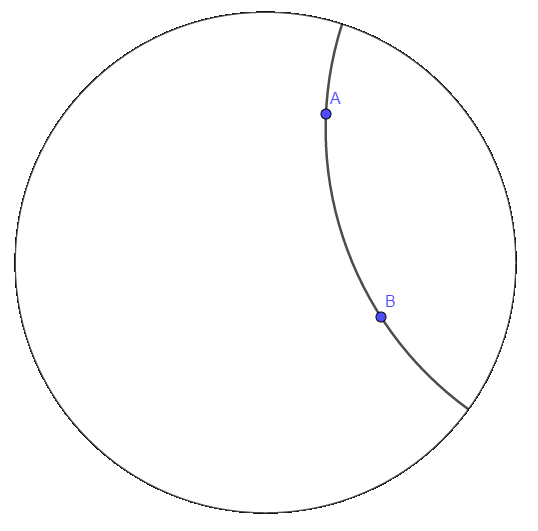
\includegraphics[width=0.35\linewidth]{pic7}
\end{figure}
Пусть $F_a, F_b, F_c$ –– проекции точки $F$ на стороны $BC, CA, AB$.\\
Четырехугольник $F_cF_bF_a$ вписанный, поэтому $\angle FF_bF_a = \angle FCF_a$. Аналогично $\angle FF_bF_c = \angle FAF_c$. Точки $F_a, F_b, F_c$ лежат на одной прямой тогда и только тогда, когда $\angle FF_bF_c = \angle FF_bF_a$, что равносильно $\angle FAF_c = \angle FCF_a$. Откуда следует что точка $F$ лежит на описанной окружности треугольника $ABC$. 
		